\section{Procedural Terrain Generation Techniques using Evolutionary Algorithms}

!!! Images need repositioning !!!

\begin{figure}[htb]
	\centering
	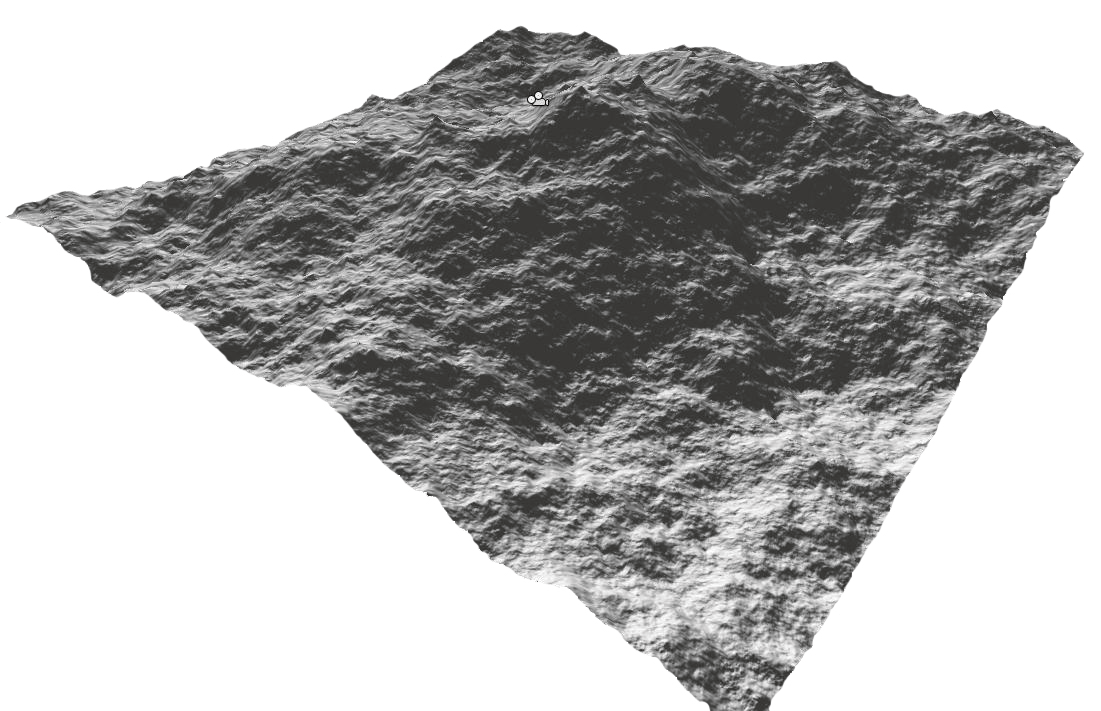
\includegraphics[width=\linewidth]{RZL12/06256610_1.png}
	\caption{Example for terrain generation by fractal subdivision}
	\label{fig:frag_subdev}
\end{figure}

\begin{figure}[htb]
	\centering
	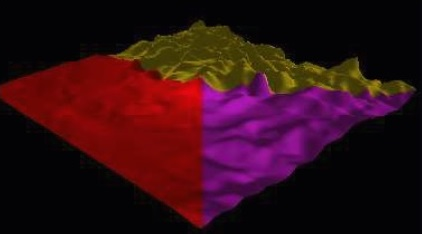
\includegraphics[width=\linewidth]{RZL12/tz76jt7ut.jpg}
	\caption{Example of results with the algorithm from \cite{ong2005terrain} and \cite{saunders2006realistic}}
	\label{fig:tag15}
\end{figure}

\begin{figure}[htb]
	\centering
	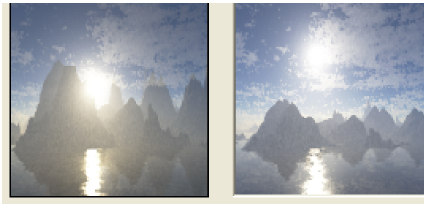
\includegraphics[width=\linewidth]{RZL12/5zr45zr6z5.png}
	\caption{Example of results with the algorithm from \cite{walsh2011use}}
	\label{fig:tag17}
\end{figure}

\begin{figure}[htb]
	\centering
	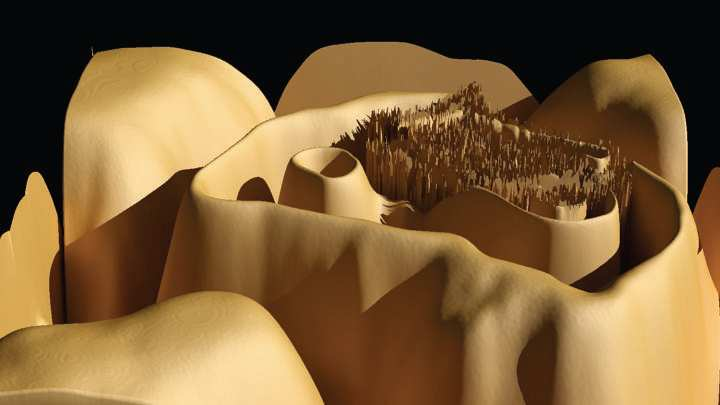
\includegraphics[width=\linewidth]{RZL12/hfhhf.jpg}
	\caption{Example of results with the algorithm from \cite{frade2009breeding}}
	\label{fig:tag19}
\end{figure}

\begin{figure}[htb]
	\centering
	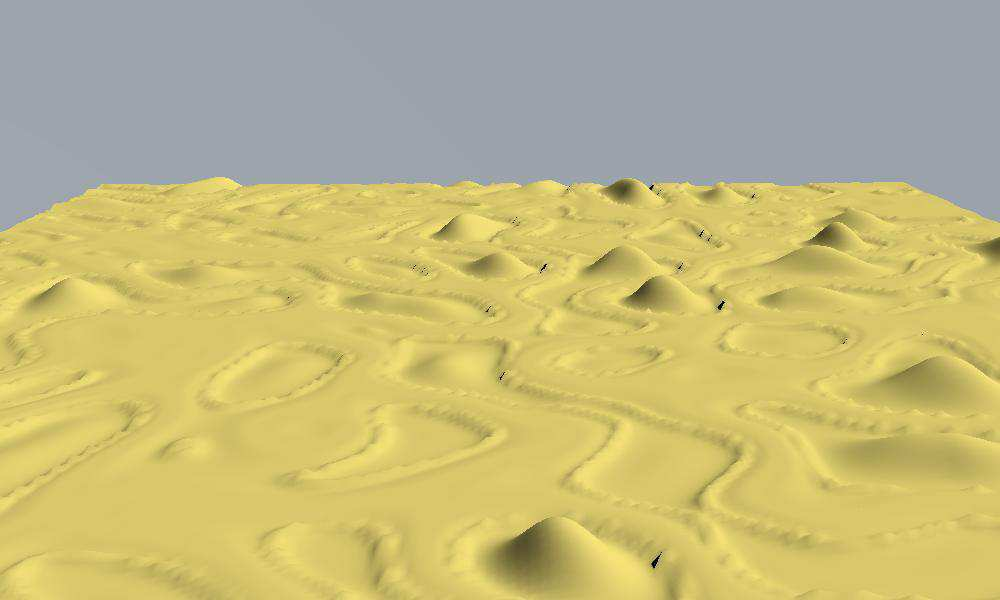
\includegraphics[width=\linewidth]{RZL12/06256610.jpg}
	\caption{Example of results with the algorithm from \cite{frade2010evolution2}}
	\label{fig:tag21}
\end{figure}

\begin{figure}[htb]
	\centering
	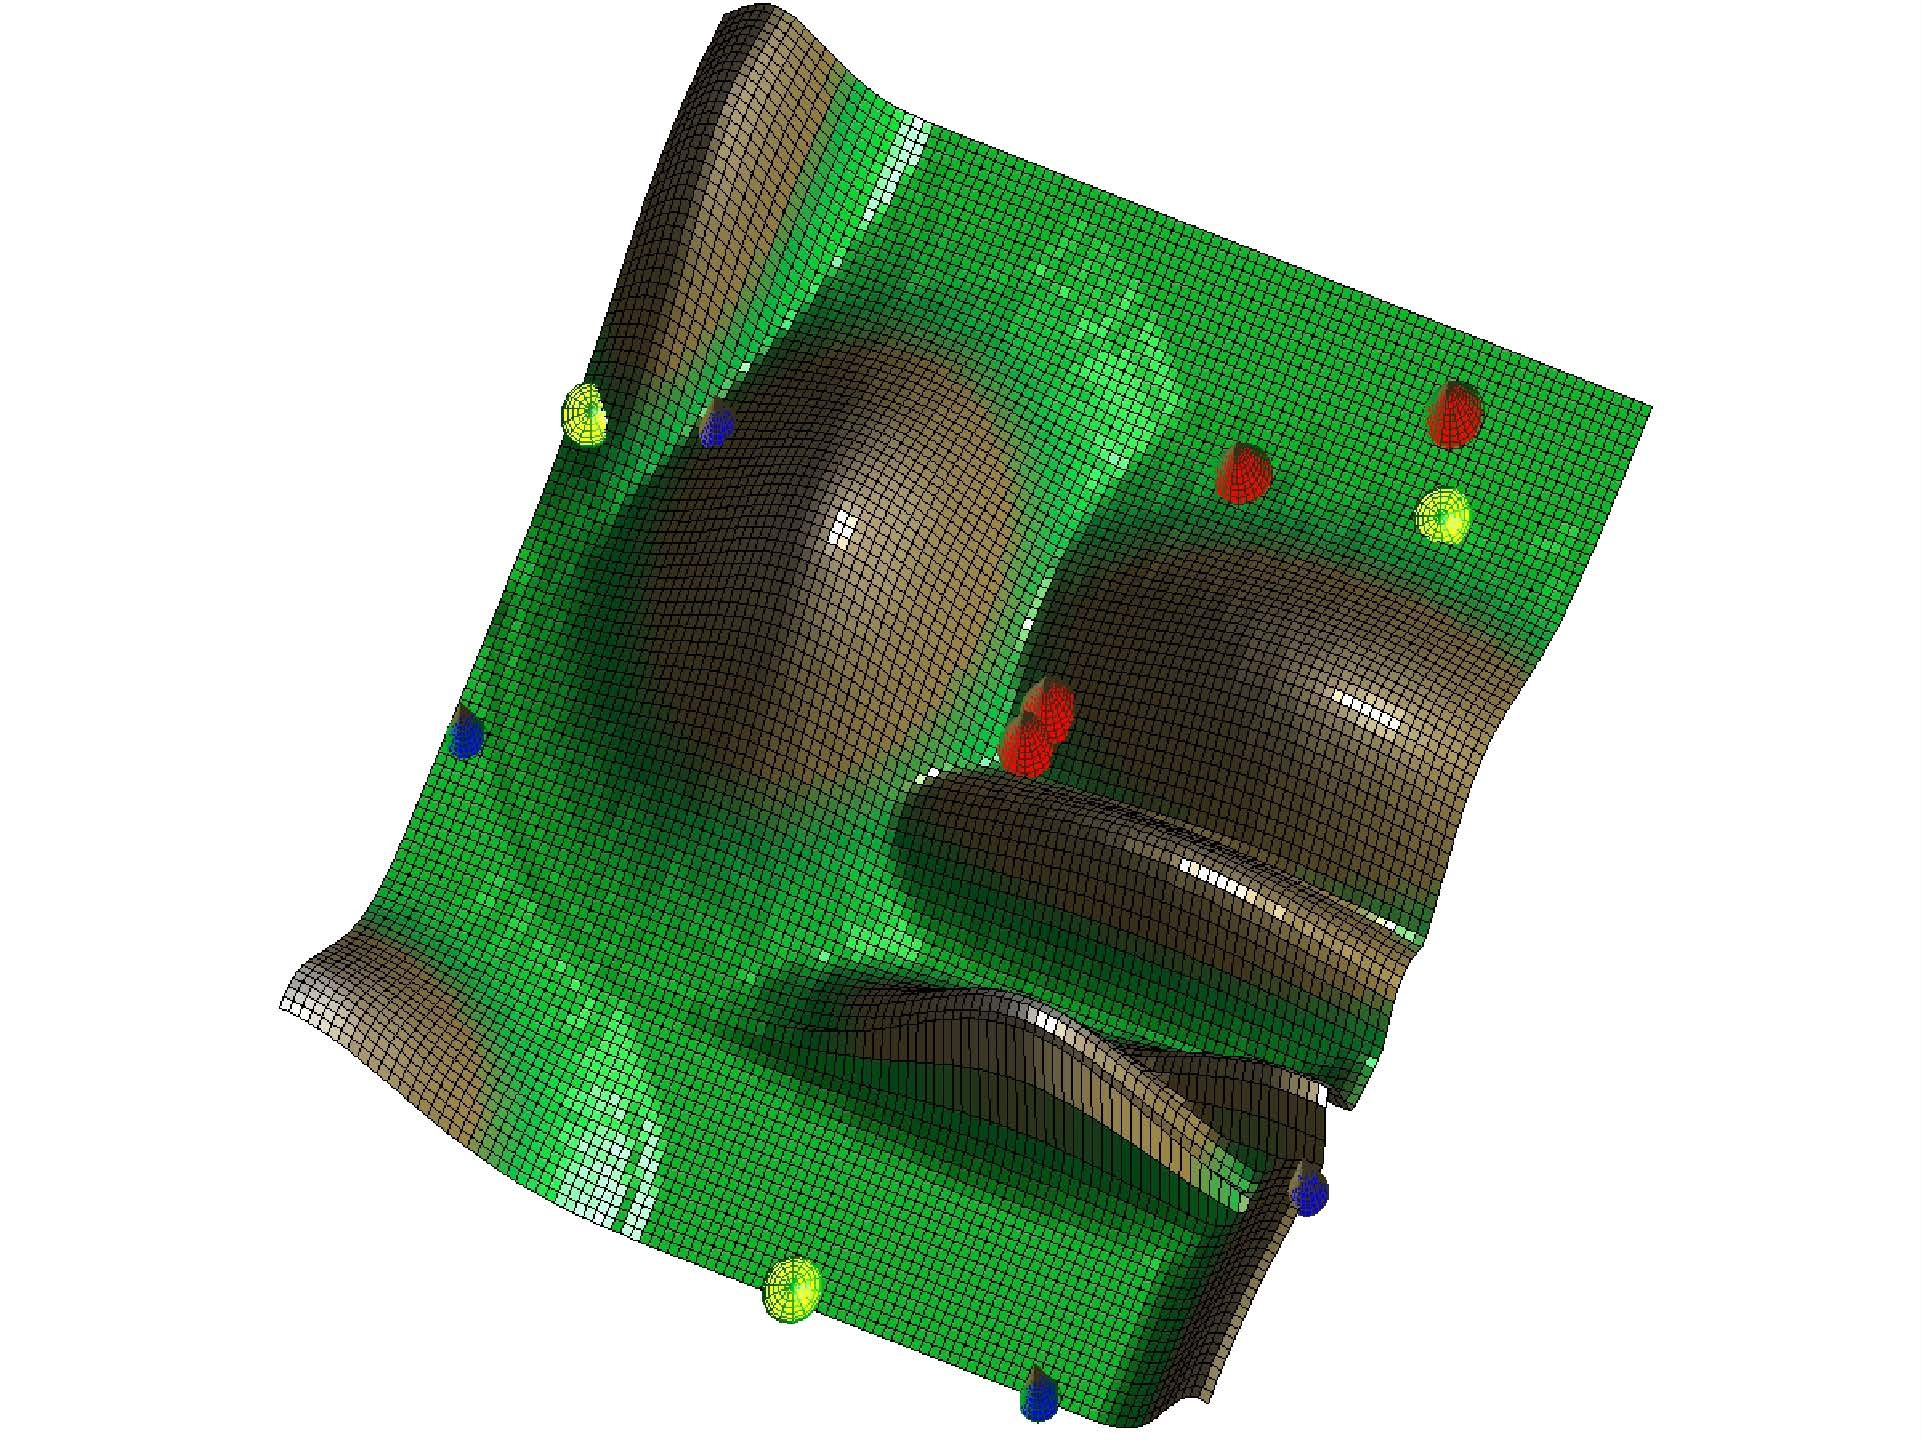
\includegraphics[width=\linewidth]{RZL12/rthrhrh.jpg}
	\caption{Example of results with the algorithm from \cite{togelius2010towards}}
	\label{fig:tag23}
\end{figure}

\begin{figure}[htb]
	\centering
	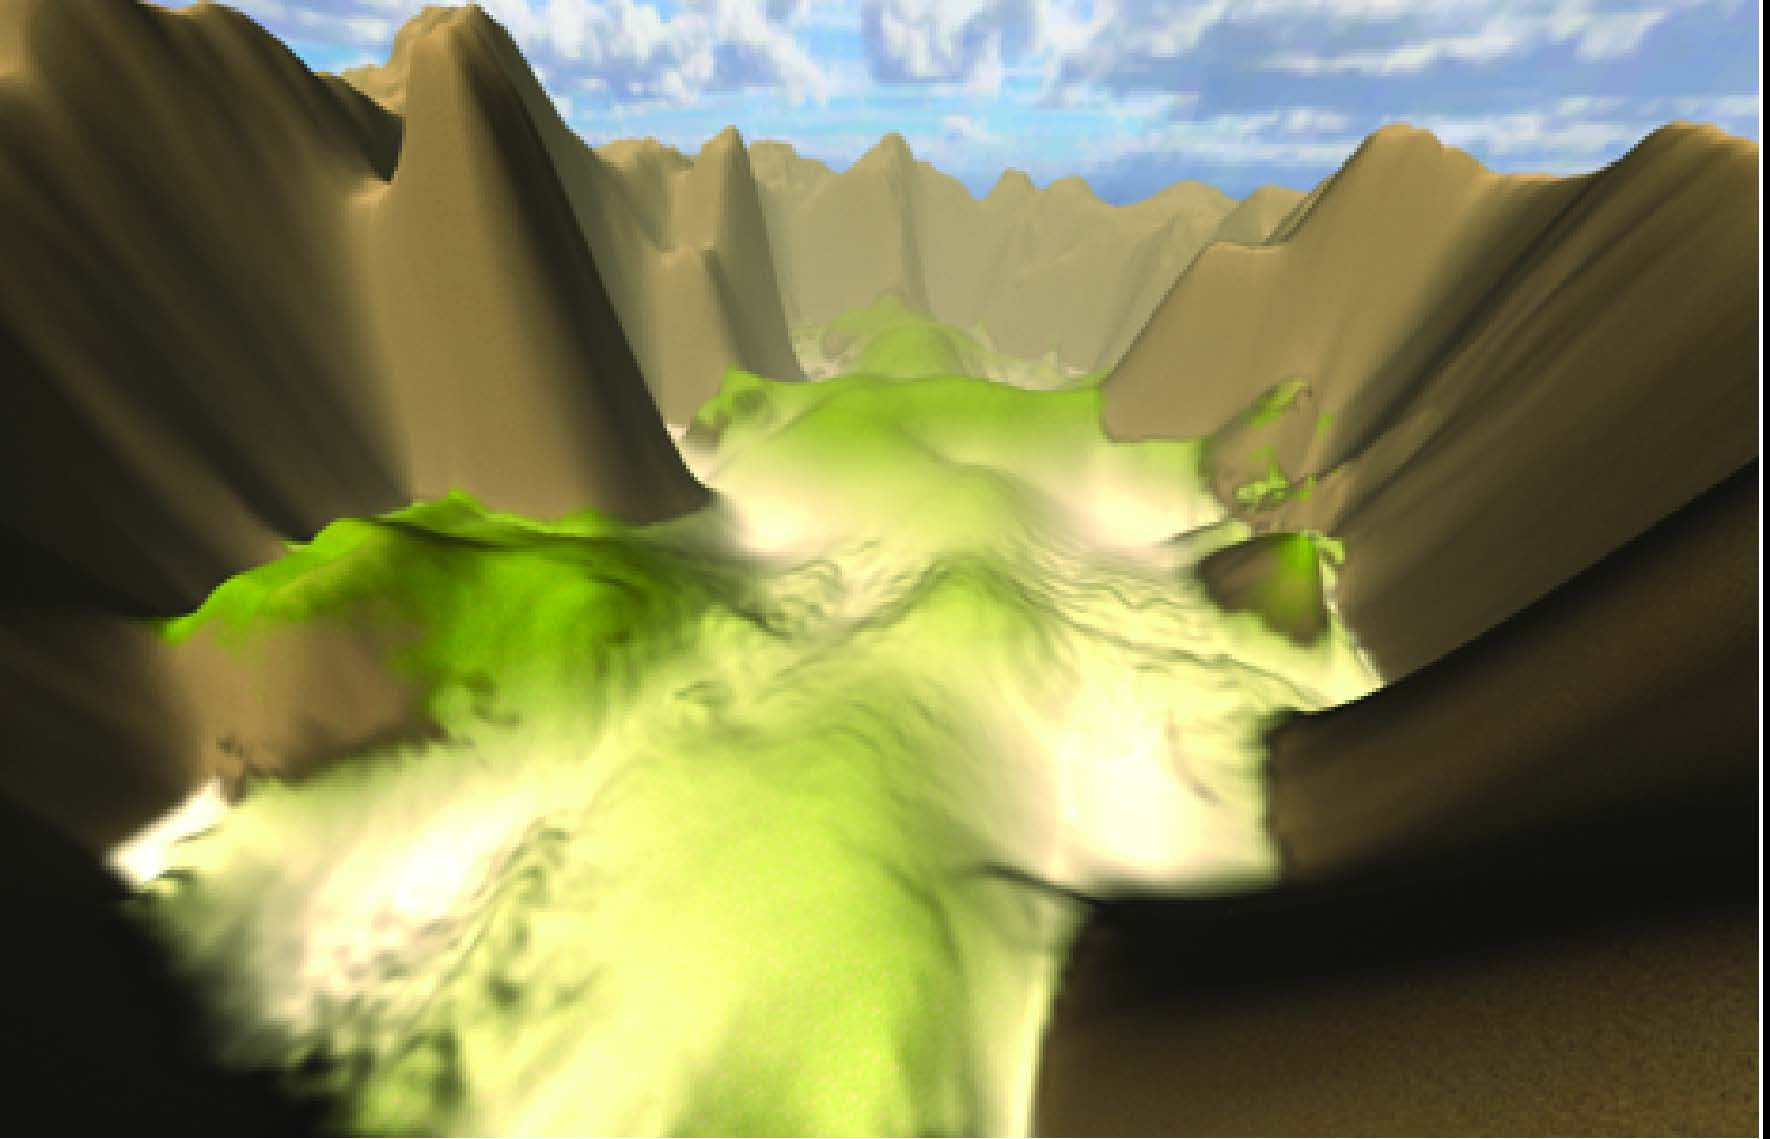
\includegraphics[width=\linewidth]{RZL12/sjrjsrtr6zsr6z.jpg}
	\caption{Example of results with the algorithm from \cite{raffe2011evolving}}
	\label{fig:tag25}
\end{figure}

This paper \cite{raffe2012survey} is rather a state of the art report itself than an actual scientific publication, since there are no novel approaches or techniques presented here. Nevertheless this paper gives us a great insight to a variety of different techniques and approaches we have been able to discuss here yet. Furthermore the viewpoint from the authors is fundamentally different to most of the other papers which have been mentioned so far.

This paper completely discards things like physical correctness and/or plausibility, and entirely focuses on algorithms ant techniques for creating terrain for game-environments. The first big difference that comes with that focus is the fact, that he only data structure used here are hight maps. Since physical correctness or even the possibility of simulating erosion processes or something like that are completely to be irrelevant in this scenario, it would not make much scene to deal with the before-mentioned downsides of voxel representations.

\subsection{Different types of algorithms}
The applied techniques for generating a feasible terrain for game can be categorized as two different types:
\begin{itemize}
	\item Fractal Subdivision 
	\item Evolutionary Algorithms
\end{itemize}

Algorithms categorized as the 1st type, have been used for many years already. An illustrative example can be seen in figure \ref{fig:frag_subdev}. The technique is clearly the older one of the two mentioned, bus is is also well researched and a lot of established algorithms and variations of it exist. The passible user input is usually controlled through a variety of parameters taken into account by the formulas used. Examples for such parameters would simple be the number of specific terrain features (mountains, cliffs, etc.) \cite{raffe2012survey}. As it can be easily imagined, this makes the amount of possible control through user interaction during the generation process quite small.

In contrast to that, the 2nd type - Evolutionary Algorithms - are a rather new field of research. The techniques rely on the random output of a variety of well established techniques for that purpose (fractals for example). An example terrain generated with the technique of \cite{togelius2010towards} can be seen in figure \ref{fig:tag23}. User interaction can be much potentially much greater here since there are a variety of different fitness functions used in evolutionary algorithms. In addition to that fact, the defining of many input parameters and the randomly generated output which can repeated several times, these techniques perform much better then fractal subdivision-approaches when it comes to user-interaction. Like the title of this paper suggests, this type of algorithms well be looked upon more closely in the following part of this paper.

\subsection{Evolutionary Algorithms}
In this state of the art report several different papers are described, evaluated and compared. Many of the presented methods have already been incorporated and in several popular computer games probably known by most of us. One important fact to consider is, that not every technique can be used for every game since different games also have different requirements for the terrain to be generated. For a 1st person shooter is might be no problem if a pattern repeats itself on a rather small-scaled map, while it would be a huge obstacle for an RPG where the player should be motivated to explore new areas of the terrain \cite{raffe2012survey}. In both these cases accessibility - so that most parts of the terrain can be traversed by the player's character - is very important. But if we consider terrain-generation for a flight simulator for example, the requirements will be fundamentally different since terrain-traversal is not of any concern in this scenario.

\subsubsection{Modifying user-provided samples}
Many of the papers presented in this state of the are report do not really create new terrain, but rather modify or recombine user-provided sample-maps. In one case (\cite{walsh2010terrain} followed by \cite{walsh2011use}) this is done by simply modifying the given terrain by applying/changing different input parameters (see figure \ref{fig:tag17}). This as of cause one big advantage: the resulting terrain is quite sure to fit the same requirements as the input-terrain did. In addition to that the modifications are very controllable by the user.

In another case \cite{raffe2011evolving} the user-provided sample-terrains (the more the better) are decomposed into many smaller patches, which are then recombined in different positions to a completely new terrain (an example can be seen in figure \ref{fig:tag25}). The possibility if a path is relocated and where it is moved to, is stochastically determined for each patch. The quality as well as the plausibility of the resulting terrains are of cause vastly defined by the chooses patch size. One important fact to consider here is, that the patches are usually quadratic / rectangular. Therefore is can be quite difficult - if not impossible - to generate triangular terrain features with this techniques.

An advantage of both those techniques and many other like them, is the simplicity of generating new maps. This can be easily done automatically without big computational effort, as well as from an unexperienced user in a map-editor for example. The big downside however, is the bad expiration of the solution space. Since every possible result from such techniques must be present in at least one of the user-provided samples, the resulting "new" terrain is also limited obviously.

\subsubsection{Generating terrain from srach}
Of cause there also are some techniques aiming to generate completely new terrains from scratch. For example in the technique used in \cite{ong2005terrain} and \cite{saunders2006realistic}, a user-provided sketch is used to generate a first 2D outline (see figure \ref{fig:tag15}). After that a hight map is generated from that data. The resulting terrain can then be modified further and be refined by the user interactively, with control points located in the terrain surface. With this interactive 2-phase approach the user keeps full control of basically all the input parameters, while still effortlessly generating a completely new terrain automatically.

Another technique is even capable of generating new terrain without any user-samples in the 1st place (see figures \ref{fig:tag19} and \ref{fig:tag21}): In the approach presented in \cite{frade2009breeding},\cite{frade2010evolution1},\cite{frade2010evolution2} and \cite{rodrigues2010development}, a stochastic noise algorithm is used to generate base hight maps. In this technique a special hight function is applied to each vertex, working with a tree of operands. An obvious problem here is the fact, that is can not be guaranteed that the resulting terrain is player-traversable (a player-avatar can walk to most of the terrain-area). Since this is quite an important and therefore critical criteria for most game-application an accessibility measurement was introduced in later implementations. In that way it's possible to generate usable maps for a variety of games, where the player can walk all across the map.

Both of these techniques have the big advantage of using the solution space quite well \cite{raffe2012survey}. But since no sample-terrains are used which already fit the required constraints, is has to be assured that the resulting terrain is usable separately.

\subsection{Performance}
As all different approaches have their own up- and downsides, it is hard to objectively compare them. The decision which algorithms to use will more likely depend of the requirements for the terrain-generation process, the number and type of constraints necessary, and the level of user-interaction desired during the process. As far as the performance of the mentioned techniques go: Unfortunately neither in the reviewed state-of-the-art report itself, nor in the underlying papers presented there, any significant, comparable performance measurements usable for our purpose here can be found. But since all presented techniques solely rely on working in hight field data is can be assumed that all mentioned approaches and algorithms are suitable for realtime interaction.